\documentclass[12pt]{article}
\usepackage[utf8]{inputenc}
\usepackage[margin=1.1in]{geometry}
\usepackage{setspace}
\usepackage{graphicx}
\title{Synthesizer Documentation}
\author{Adithya Shastry and Danny Farr}
\date{January 2020}

\begin{document}
\maketitle
\newpage
\tableofcontents
\newpage
\section{Overview}
The goal of our project was to create the It only consists of a Voltage Controlled Oscillator that produces different waveforms and different frequencies of sound. This is all done using switches and dials. The central part of the entire circuit is the LM555 chip which takes the DC input we have given it and converts it to AC in the form of a square wave. We then used integrated circuits to produce the other wave forms we wanted to produce. The inputs to the LM555 chip allowed us play around with the frequencies of notes. 
\section{Hardware Requirements}
The hardware requirements for the project can be seen in table \ref{Parts List}
\begin{table}[h!]
\centering
\begin{tabular}{|l|l|}
\hline
\textbf{Part Name} & \textbf{Amount} \\ \hline
Protoboard & 1 \\ \hline
LM555 & 1(have backups) \\ \hline
Bread Boards & 2 \\ \hline
Digital Multi Meter and cables & 1 \\ \hline
2 Way Switches & 2 \\ \hline
Push Buttons & As many as you want keys \\ \hline
Various Resistors & Will depend on frequencies desired \\ \hline
10k$\Omega$ Resistor & 3 \\ \hline
1k$\Omega$ Resistor & 2 \\ \hline
1M$\Omega$ Resistor & 1 \\ \hline
100k$\Omega$ Resistor & 2 \\ \hline
Osciliscope & Not Required \\ \hline
100k$\Omega$ Potentiometer & At least 1 to bend notes \\ \hline
LM741 & 2(have backups) \\ \hline
Speaker & 1 \\ \hline
Wires & Many \\ \hline
0.1 $\mu F$ & 2 \\ \hline
0.01 $\mu F$ & 2 \\ \hline
10V Voltage Source & 1 \\ \hline
\end{tabular}
\caption{Table of Hardware requirements}
\label{Parts List}
\end{table}
%Should be just a list of the actual components we needed to build our synth
\section{Hardware Implementation}
The Schematic diagram can be seen in figure \ref{schematic}. For more reference of how we came to building this circuit as well as what each part of the schematic does please consult our lab journal that details the entire process of creating this synthesizer.
\begin{figure}[h!]
    \centering
    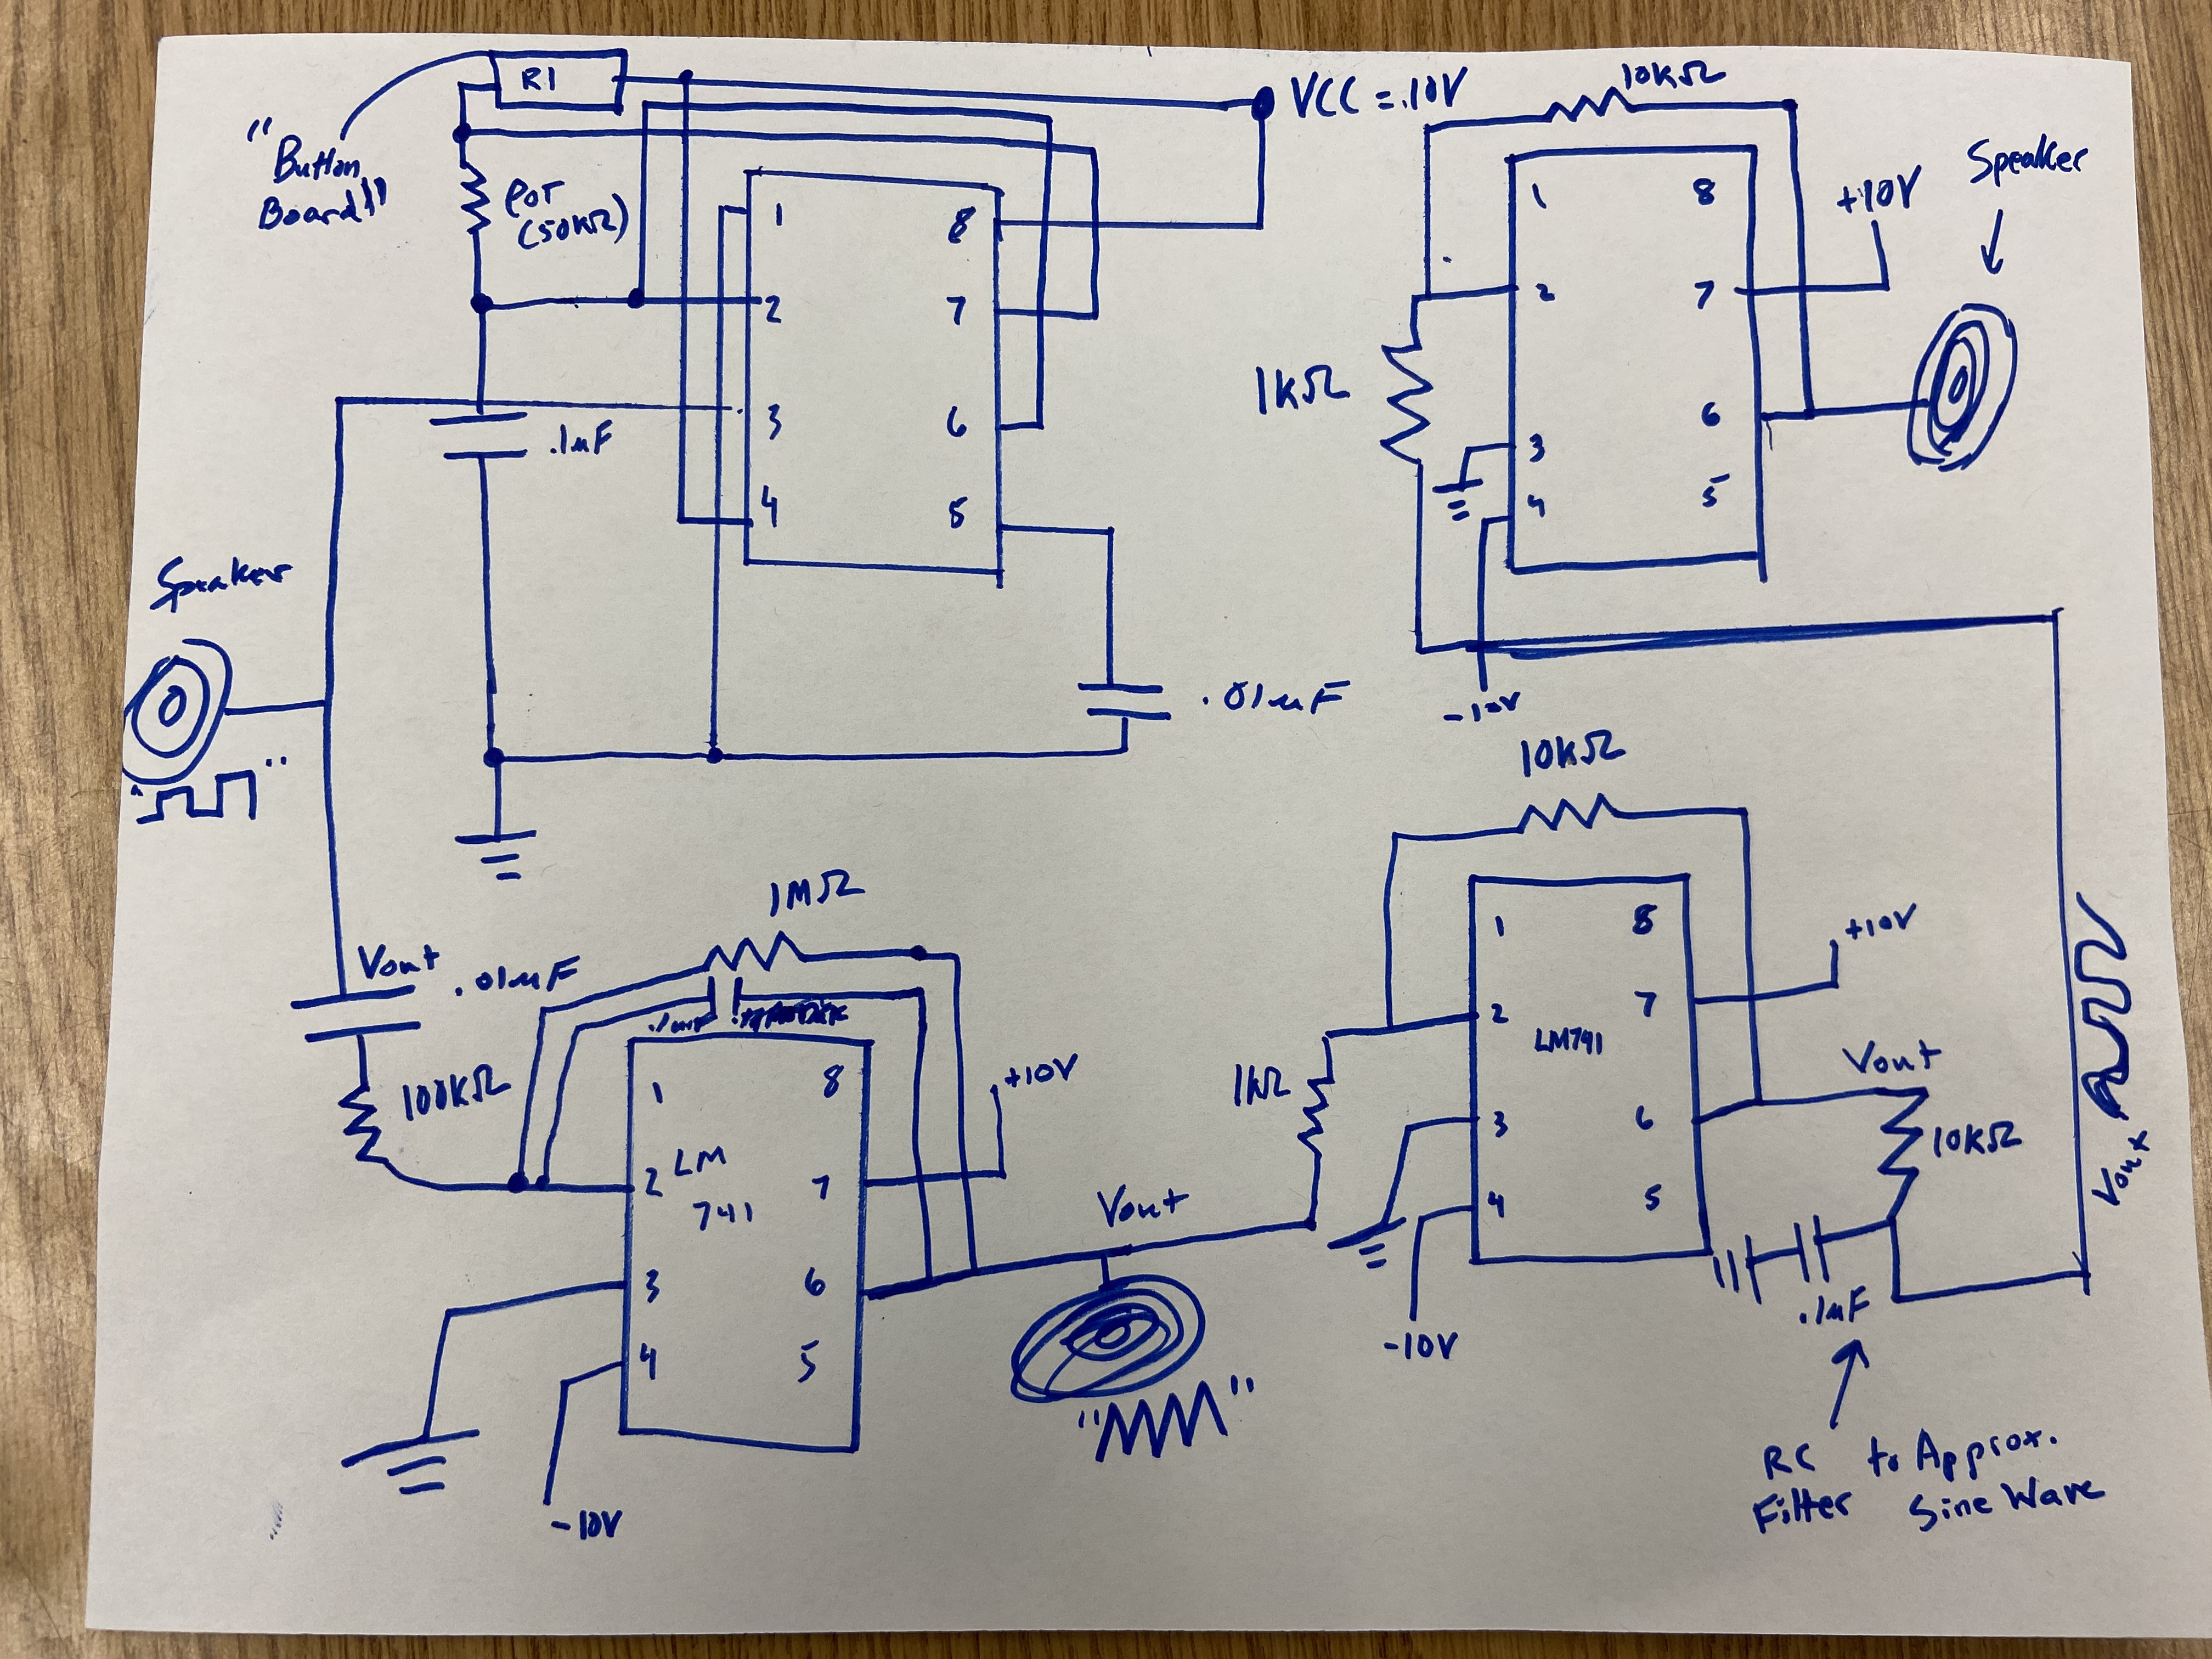
\includegraphics[scale=0.1]{schematic.jpg}
    \caption{This is the Schematic for the synthesizer}
    \label{schematic}
\end{figure}
\newpage
Note that the button board was simply a series of buttons connected in parallel to both the input and the output. 
We ended up soldering to a perfboard the buttons and the resistors since the buttons kept popping out of the breadboard we had attached them to. This was done using a non-copper plated perfboard and therefore required wires to conduct current. The button side of the board can be seen in figure \ref{buttons} and the underside of the board can be seen in figure \ref{botbuttons}
\newpage
\begin{figure}[h!]
    \centering
    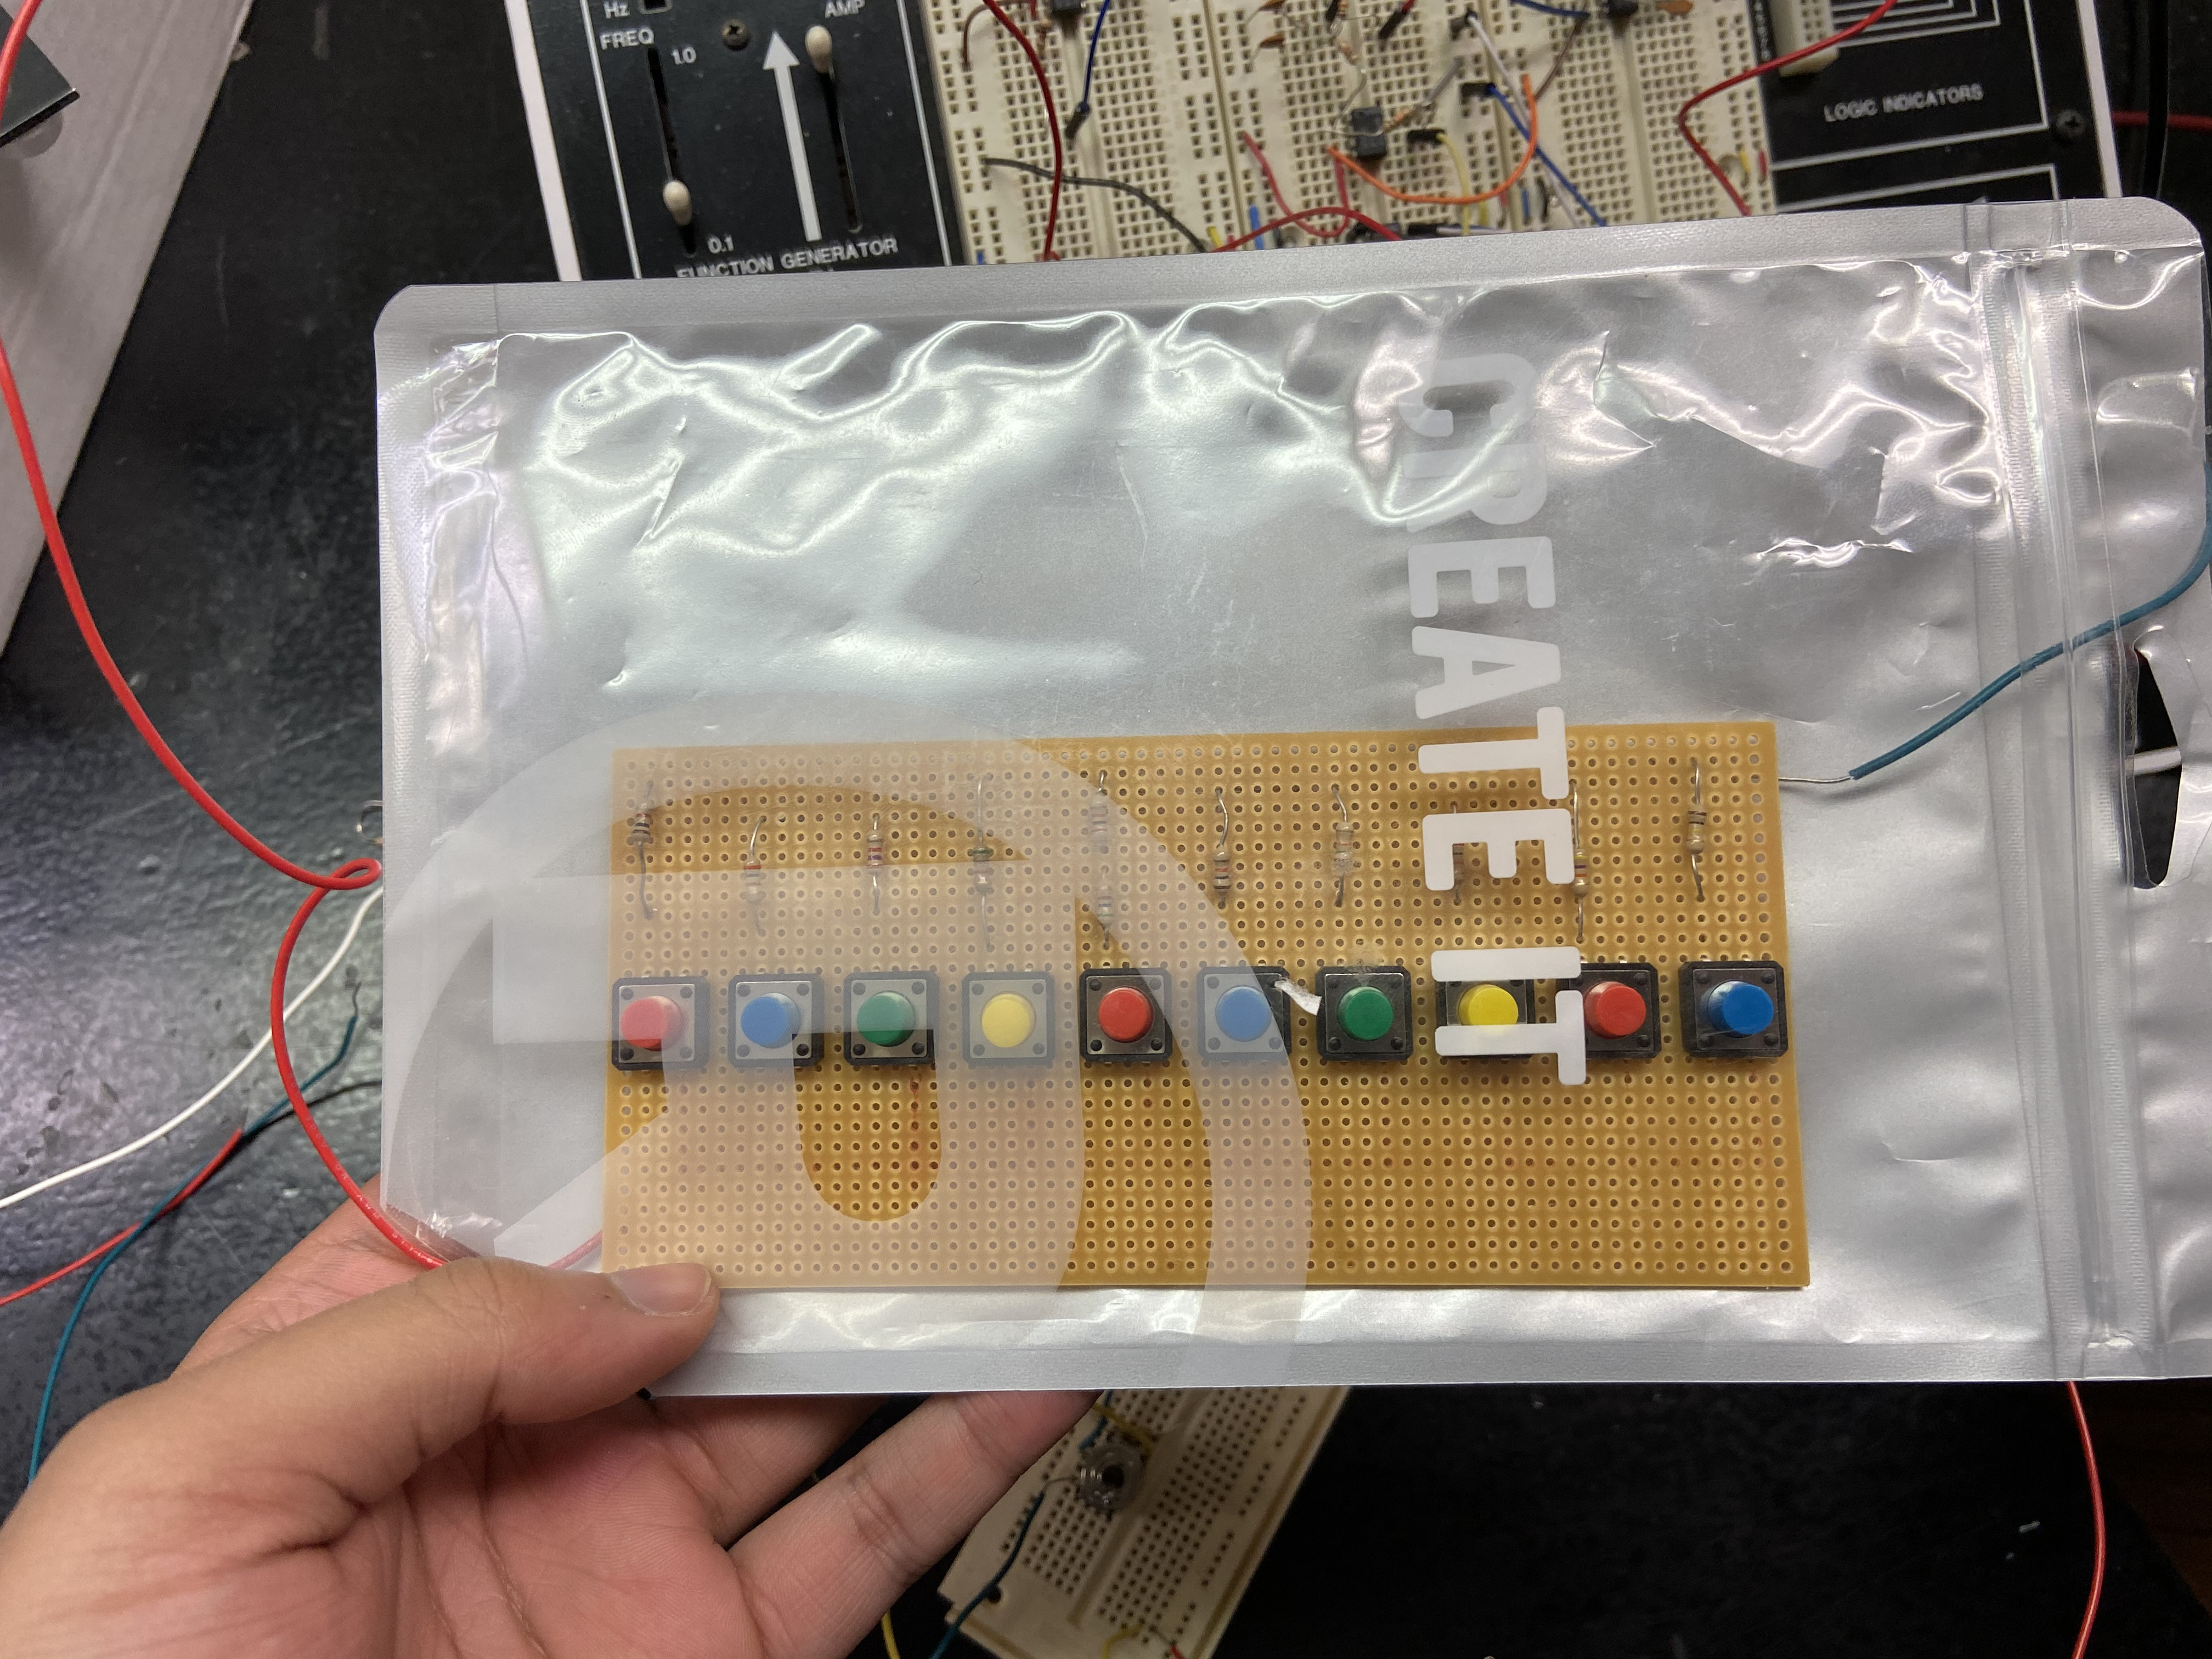
\includegraphics[scale=0.1]{buttons.jpg}
    \caption{Buttons to play notes}
    \label{buttons}
\end{figure}
\begin{figure}[h!]
    \centering
    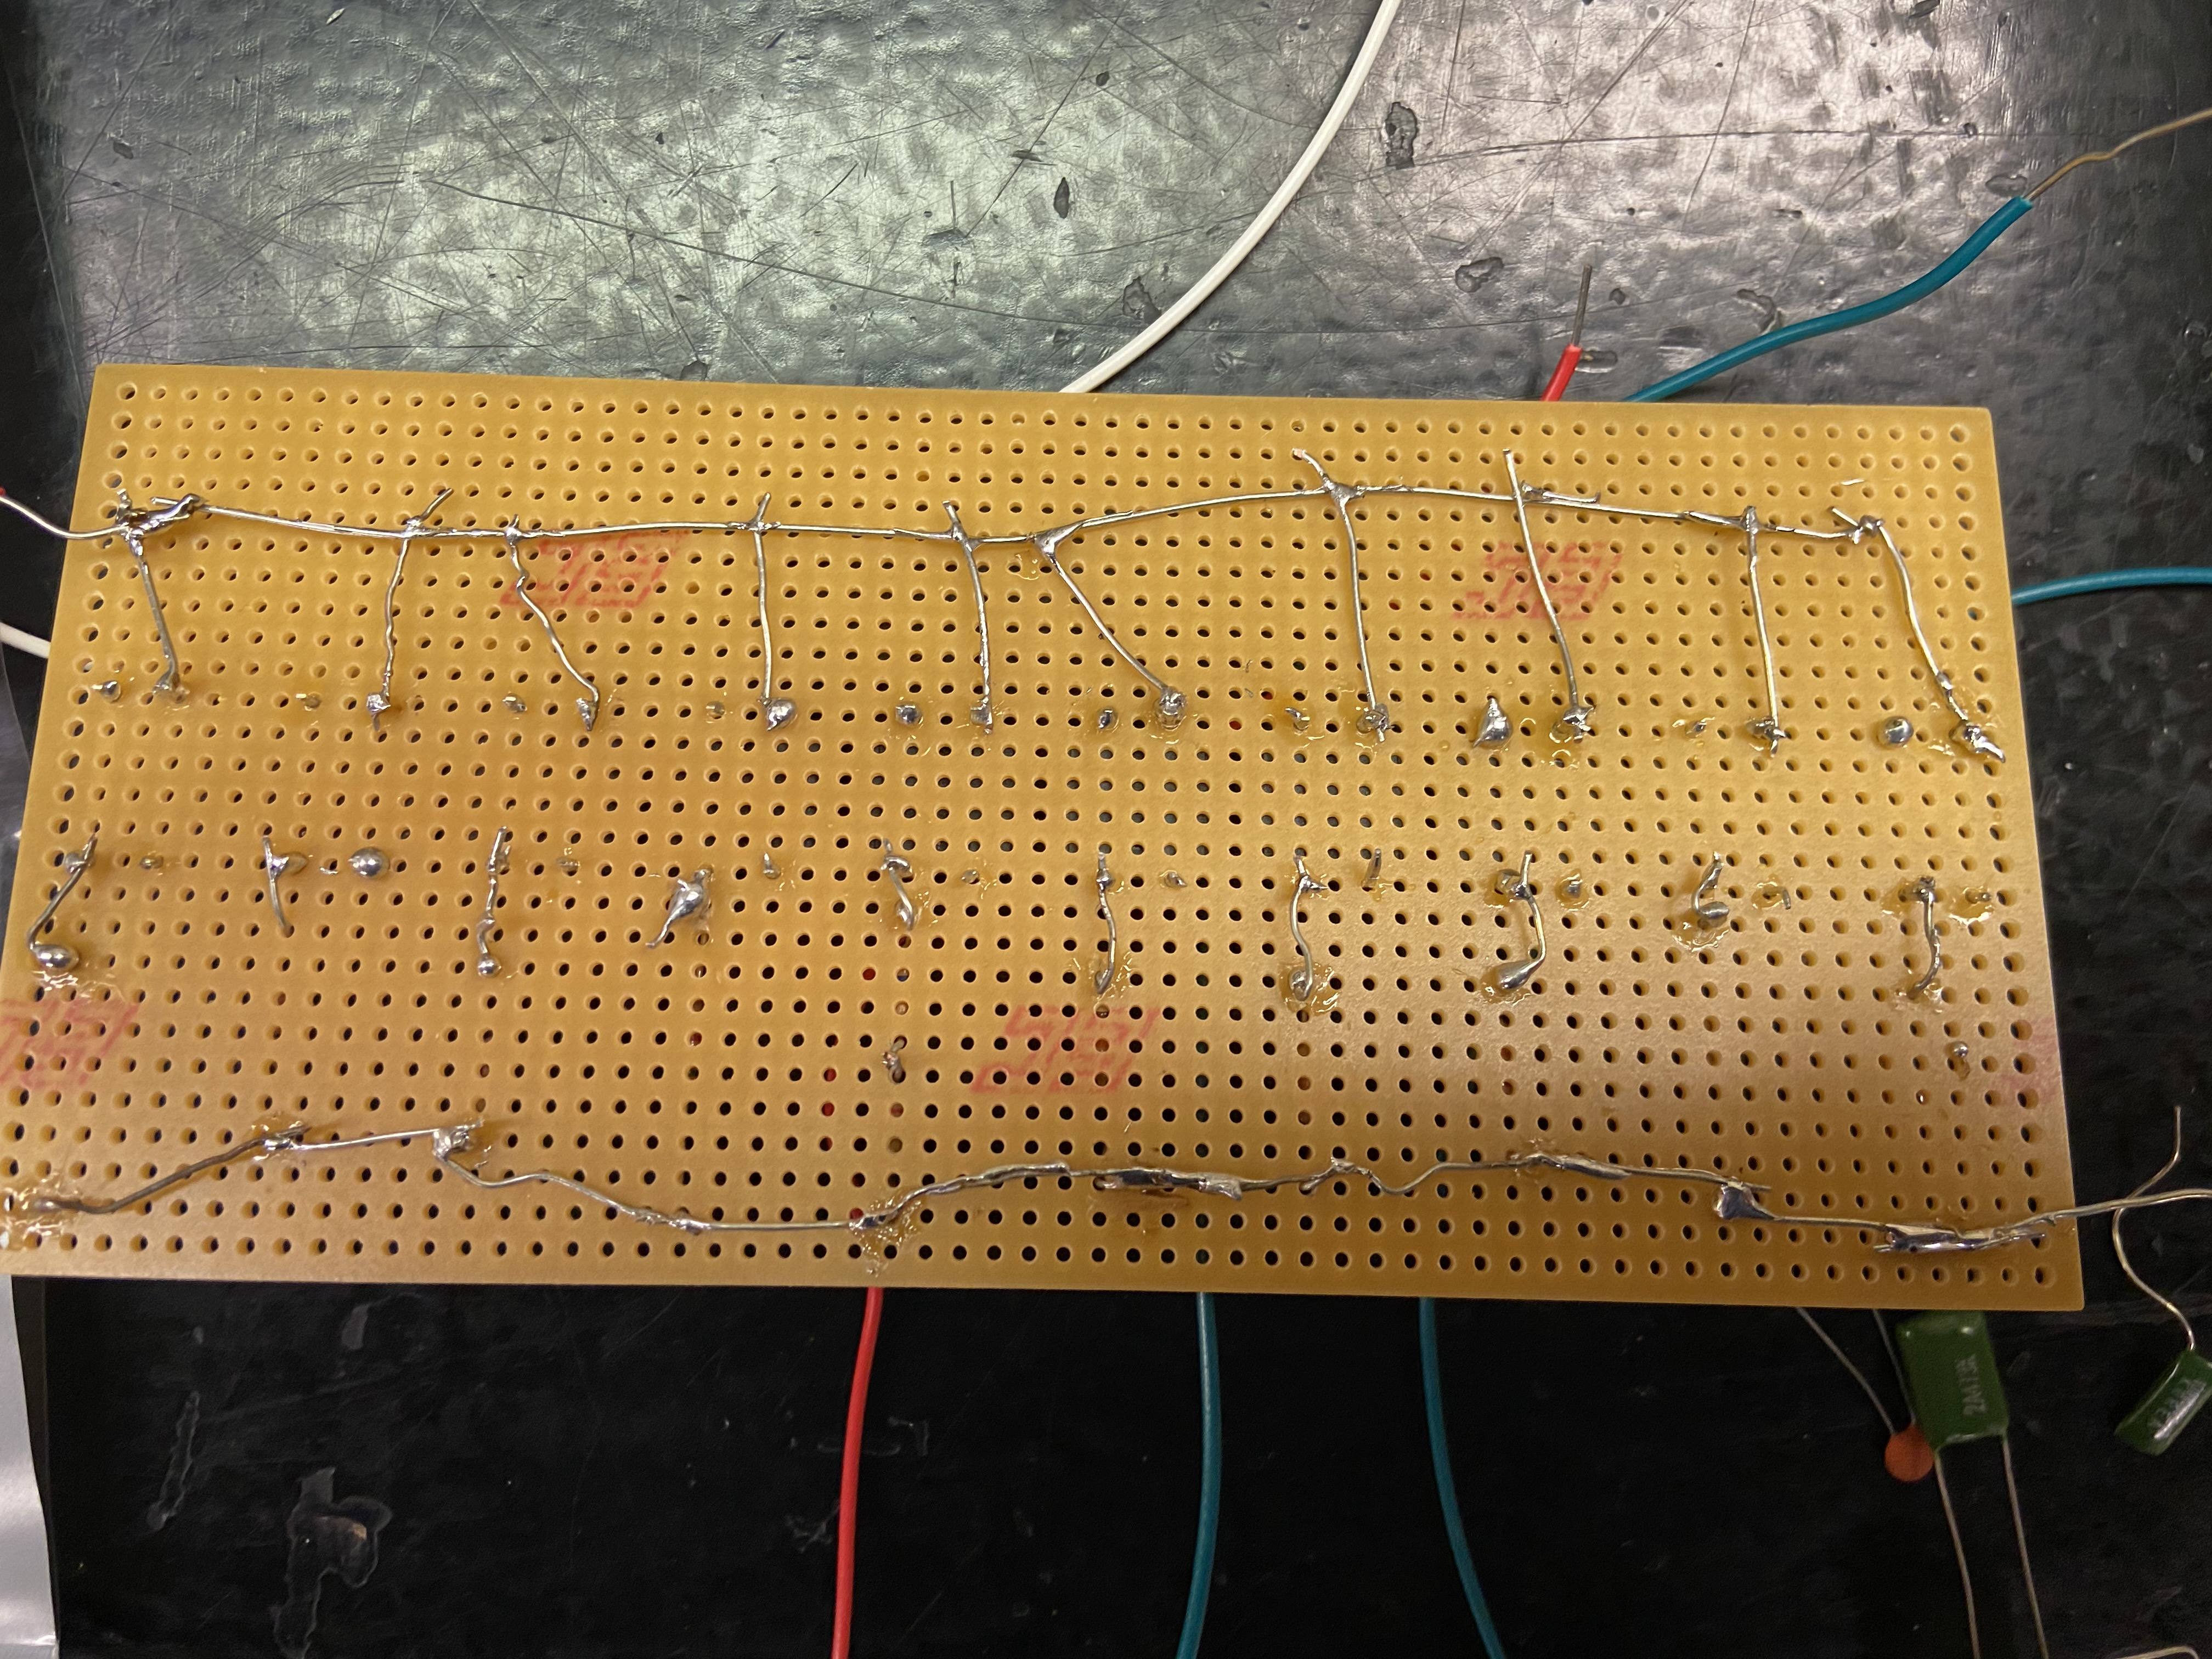
\includegraphics[scale=0.1]{botbuttons.jpg}
    \caption{Soldering for the buttons}
    \label{botbuttons}
\end{figure}
\newpage
With all of that said, the final version of our project can be seen in figure \ref{complete}
\begin{figure}[h!]
    \centering
    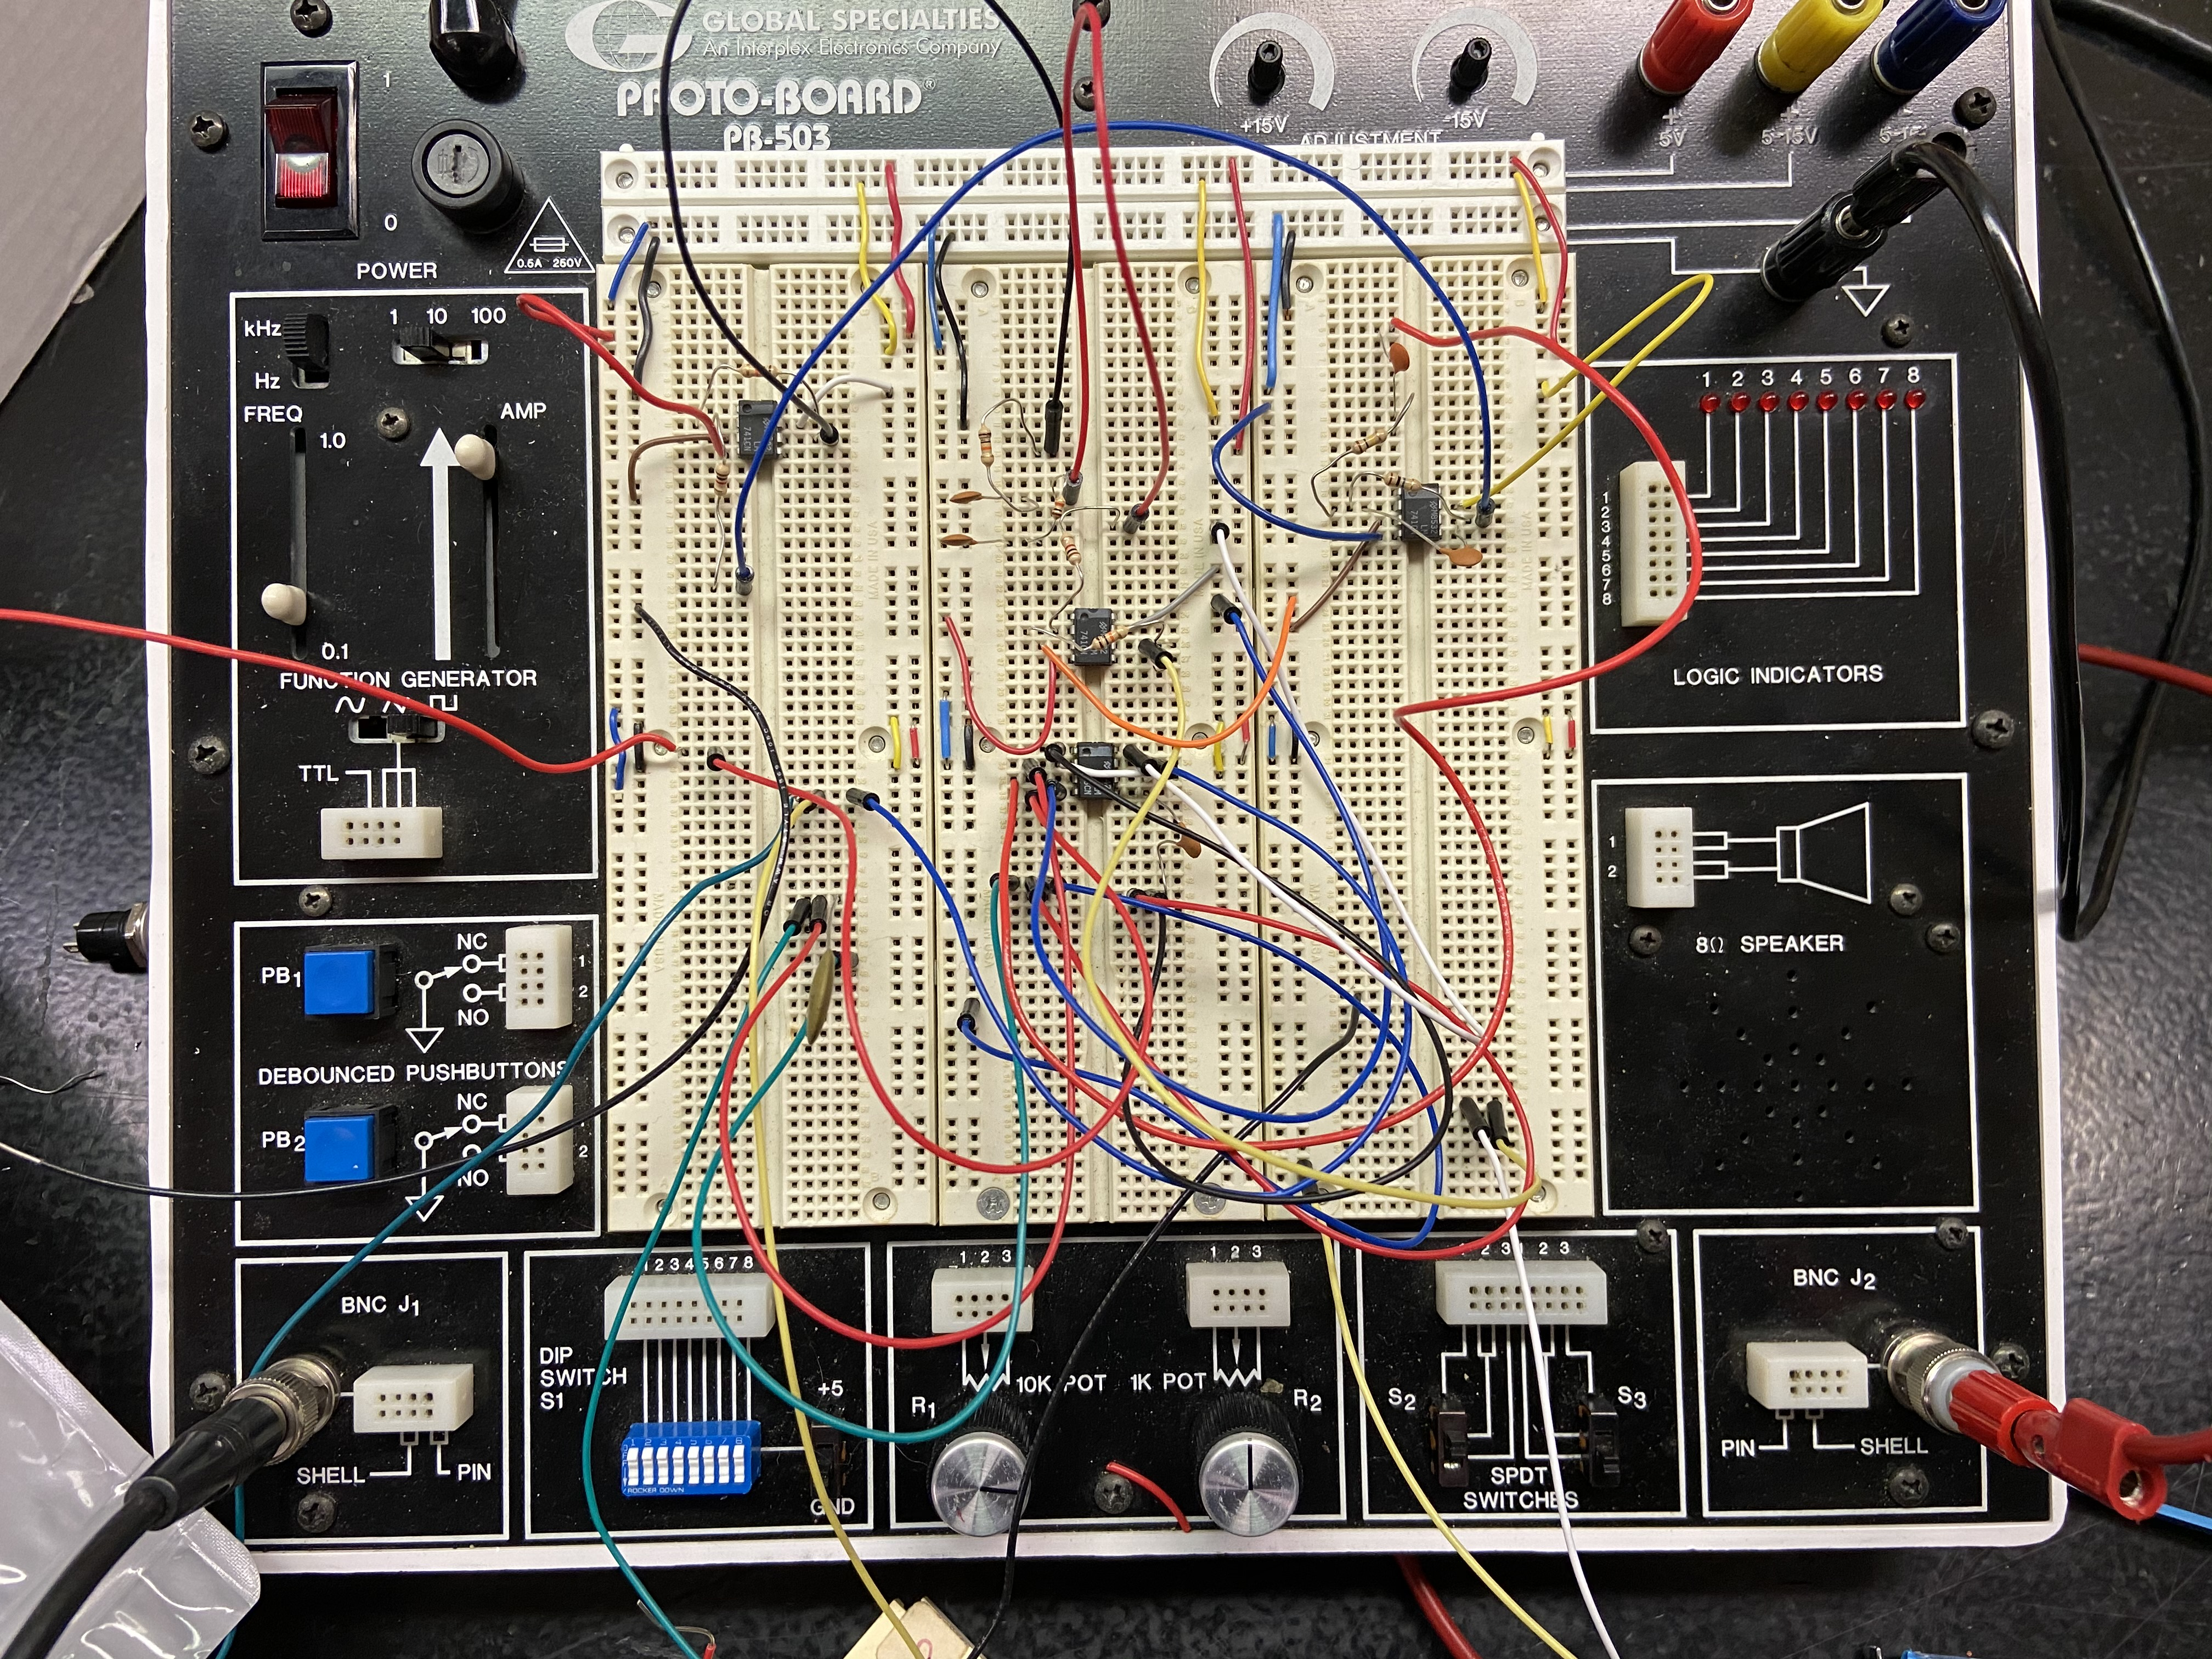
\includegraphics[scale=0.1]{complete.jpg}
    \caption{The Complete Protoboard set up}
    \label{complete}
\end{figure}{}
\newpage
%Include some things to look out for
%Include a schematic
%the call the schematic "schematic" to create the correct reference below
%Include pictures 
\section{Testing and Further Improvements}
% Write things you can improve the synthesizer 
% Write a bit about how we tested the device and what things can be changed in order to change the noise actually outputted
The device was mainly tested by using the speaker provided on the protoboard and an oscilloscope, but the oscilloscope is not required. The speaker was used to understand if a note was actually being played when we pressed a button. We found the specific resistances we wanted based on a tuner app that we found on the app store(Please note: this is only needed if you want to produce frequencies similar to specific notes on the piano). Changing the capacitor used in series with the keys and the variable resistor( as seen in figure \ref{schematic}) can be changed to move the entire frequency range up or down. We used this in order to get the output of the LM555 timer to output in a hear able range. 

The oscilloscope was used to understand whether the output was actually of the waveform we wanted. This was a major part of the time used to build the project, but since we have already given schematic diagrams for the sine wave and triangle wave generators this should not be such a hassle, therefore the oscilloscope is not really required for this specific build. The entire building and testing process can be seen in the lab notes attached to the end of this document

Further improvements for this synthesizer are to possibly create the sawtooth waveform, more modules for the synth such as an envelop generator, sample and hold, sequencer, and many more. There is simply no end to the amount we can do with this baseline part of the synth.
\section{Conclusion}
In conclusion, this was a great project to build because it was a good way of understanding the inner workings of the LM555 timer, OP amps, and many other electrical components and circuits. We hope to rebuild this circuit after this class and add on some more modules to make cooler sounds!


\section{Appendix I:Lab Notes}
Access to our Lab Journal can be gained using this link: https://tinyurl.com/stgsbq4

\end{document}



